% AASTeX v6.2
%\documentclass[preprint]{aastex62}

% ApJ Format
\documentclass[iop,revtex4,twocolumn,apj,numberedappendix,appendixfloats]{emulateapj}
\usepackage{apjfonts}
% Hyperlinks & Bookmarks
\usepackage[pagebackref=false,colorlinks=true,citecolor=blue,linkcolor=blue,breaklinks=true,bookmarks=true]{hyperref}
\usepackage{amsmath}
\usepackage{comment}

% Units
\newcommand{\kms}{km~s$^{-1}$}
\newcommand{\msun}{$M_{\odot}$}
\newcommand{\msunyr}{$M_{\odot}~{\rm yr}^{-1}$}
\newcommand{\lsun}{$L_{\odot}$}
\newcommand{\ergs}{erg~s$^{-1}$}
\newcommand{\cmsq}{cm$^{-2}$}
\newcommand{\um}{$\mu$m}
\newcommand{\uJy}{$\mu$Jy}
\newcommand{\sqdeg}{deg$^2$}
\newcommand{\lx}{$L_{\rm X}$}
\newcommand{\lmir}{$L_{\rm 12\mu m}$}
\newcommand{\loiii}{$L_{\rm [OIII]}$}
% Emission lines
\newcommand{\Ha}{H$\alpha$}
\newcommand{\Hb}{H$\beta$}
\newcommand{\OII}{[O\,{\sc ii}]}
\newcommand{\OIIlam}{[O\,{\sc ii}]\,$\lambda$3727}
\newcommand{\SII}{[S\,{\sc ii}]}
\newcommand{\OIII}{[O\,{\sc iii}]}
\newcommand{\OIIIlam}{[O\,{\sc iii}]\,$\lambda$5007}
\newcommand{\NII}{[N\,{\sc ii}]}
\newcommand{\NeIII}{[Ne\,{\sc iii}]}
% special 
\newcommand{\nod}{\nodata}

\newcommand{\angstrom}{\mbox{\normalfont\AA}}
\newcommand{\reff}{$R_{\rm eff}$}
\newcommand{\ewha}{EW(H$\alpha$)}
\newcommand{\logm}{log({\it M}/M$_{\odot}$)}
%\newcommand{\arcsec}{\prime\prime}
\newcommand{\simard}{Simard+11}

% citations
\defcitealias{Fu:2018}{Paper I} 

\usepackage{epstopdf}

\begin{document}

\title{
SDSS-IV MaNGA: The Radial Profile of Enhanced Star Formation in Close Galaxy Pairs
}

\author{
Joshua L. Steffen\altaffilmark{1}, 
Hai Fu\altaffilmark{1}, and 
MaNGA Team 
}
\altaffiltext{1}{Department of Physics \& Astronomy, The University of Iowa, 203 Van Allen Hall, Iowa City, IA 52242}

\begin{abstract}
We compare the radial profiles of the specific star formation rate (sSFR) in a sample of 220 star-forming galaxies in close pairs with those of mass-matched isolated galaxies in the SDSS-IV MaNGA survey. We find that the sSFR is centrally enhanced (within one effective radius) in interacting galaxies by $\sim$0.3 dex and that there is a weak sSFR suppression in the outskirts of the galaxies of $\sim$0.1 dex. We stack the differences profiles for galaxies in five stellar mass bins between \logm\ $=$ 9.0$-$11.5 and find that the sSFR enhancement has no dependence on the stellar mass. The same result is obtained when the comparison galaxies are matched to each paired galaxy in both stellar mass and redshift. In addition, we find that that the sSFR enhancement is elevated in pairs with nearly equal masses and closer projected separations, in agreement with previous work based on single-fiber spectroscopy.
\end{abstract}

\keywords{galaxies: star formation --- galaxies: nuclei --- galaxies: interactions --- galaxies: mass evolution}

%%%%%%%%%%%%%%%%%%%%%%%%%%%%%%%%%%%%%%%%%%%%%%%%%%%%
\section{Introduction}\label{sec:intro}

%%%Galaxy Evolution%%%
In the $\Lambda$CDM model, galaxy evolution is a hierarchical process. In this model, massive galaxies are the product of several past merger events of smaller galaxies. In fact, cosmological hydrodynamical simulations have shown that repeated merger events may be responsible for as much as $\sim$60\% of stellar mass in massive galaxies like M87 \citep[e.g.,][]{Rodriguez-Gomez:2016,Pillepich:2018}. As the galaxies undergo the merging process, the gas within the galaxies are subject to gravitational torques which perturb the morphology of the galaxies.

%%%Simulations%%%
The internal dynamics of these interacting galaxies were first modeled in the seminal work, \citet{Toomre:1972}. Since then, hydrodynamical simulations have expanded upon the N-body simulations of \citet{Toomre:1972} by modeling gas-dynamics within the galaxies. These simulations show how barred structures develop within the disks of the interacting galaxies due to the tidal torques between them \citep{Barnes:1991}. As the bars form, the gases within the galaxy's disk lose angular momentum and get funneled into the centers of the galaxies. 

When the gas-inflows impact upon the gases in the nucleus of galaxy a burst of new star formation in triggered \citep{Barnes:1996, Mihos:1996}. These gas inflows will also bring metal-poor gases from the disk into the center of the galaxy which can dilute the central metallicity \citep{Rupke:2010, Perez:2011, Scudder:2012}. The gas-inflows may also be able to make it into very center of the galaxy and trigger supermassive black hole (SMBH) accretion \citep{Capelo:2017}. 

%%%Observations%%%
Interaction induced star formation was first seen observationally in the bluer colors of peculiar galaxies in \citet{Larson:1978}. This observation has also been shown in more recent works using the single-fiber spectroscopic survey, SDSS (Sloan Digital Sky Survey) \citep{Ellison:2008, Li:2008, Scudder:2012, Patton:2013, Bustamante:2020}. From these previous works it has been shown that the strength of the star formation enhancement in the centers of paired galaxies is dependent on the stellar mass of the pairs \citep{Li:2008}, the projected separation between the pairs \citep{Ellison:2008, Li:2008, Scudder:2012}, and the mass ratio between the pairs \citep{Ellison:2008}. 

%%%Integral Field Spectroscopy%%%
The previous mentioned works using SDSS were restricted to studying the centers of the paired galaxies through 2\arcsec\ diameter optical fibers. With the recent large integral field spectroscopic (IFS) surveys, interacting galaxies can now be studied with unprecedented spatial detail. These surveys allow us to study the centers of merging galaxies more rigorously since apertures can be set to the physical scale of the galaxies instead of being bound by a fixed sky aperture. These IFS surveys will also allow us to see the extent of the centrally induced star formation and to see how the star formation in the disks of the galaxies are affected. 

Indeed, \citet{Barrera-Ballesteros:2015} used the CALIFA (Calar Alto Legacy Integral Field Area) survey to study a sample of 103 paired galaxies by varying the size of the aperture through which the \ewha\ is extracted from. In the study, \citet{Barrera-Ballesteros:2015} found a moderate enhancement to the sSFR in the centers of paired galaxies and a moderate suppression to the sSFR in outskirts of the paired galaxies. 
%
\citet{Pan:2019} used the MaNGA survey to study radial profiles of a sample of 205 paired galaxies. The enhancement to the sSFR was shown to be the strongest in the centers of the paired galaxies. This central enhancement linearly fell with increasing galactocentric radii; however, a moderate enhancement to the sSFR remain in the outskirts of the galaxies. \citet{Pan:2019} further studied the paired galaxies as a function of merger stage; from well separated pairs to post-merger galaxies. Across the different merger stages, the sSFR enhancement was greatest in close pairs with tidal features and in post-merger galaxies. This was in agreement with previous hydrodynamical simulations which showed that a burst of star formation is triggered after the first pericenter and as the two galaxies begin to coalesce \citep{Scudder:2012}. 
%
The radial profile of sSFR in post-merger galaxies has also been studied with the MaNGA survey by \citet{Thorp:2019}. The post-merger galaxies were shown to have a strong enhancement to the sSFR in their centers as well as a moderate enhancement in their outskirts. 

Where previous studies on the radial profile of the sSFR offsets in paired galaxies have focused on studying the profiles as a function of interaction stage, we will focus on the radial profile as a function of the stellar mass, projected separation, and mass ratio. As mentioned previously, these parameters have been covered by studies restricted to the nuclear region of the paired galaxies. With the MaNGA survey, we will be able to expand upon these previous studies in greater spatial detail. We will be able to see how these three parameters affect the both the level of the sSFR offsets in the centers of the paired galaxies and the offsets in the outskirts of the galaxies. We will also be able to study if any of three parameters influence the gradient of the sSFR enhancement profiles or if the gradient is preserved between different configurations. 

In our previous work, we built a sample of paired galaxies in the MaNGA survey where both components of the pair were contained within field of view of a single integral field unit \citep[][hereafter \citetalias{Fu:2018}]{Fu:2018}. We found that approximately 5.7\% of the MaNGA galaxies have a companion galaxy contained within the field-of-view of a single IFU. In this work, we will use a version of this sample updated for the recent MaNGA Data Release 16 (DR16) \citep{Ahumada:2020} and we will further supplement this with a sample of companion galaxies identified outside the field-of-view of the MaNGA IFUs. 

% Organization
This paper is organized as follows; in Section \ref{sec:data} we will discuss the properties of the MaNGA survey along with the construction of our pair and control samples, in Section \ref{sec:analysis} we will discuss how we measure star formation rates and how we build radial profiles of star formation, in Section \ref{sec:results} we study the radial profiles as a function of stellar mass, projected separation, and the mass ratio, in Section \ref{sec:disc} we compare our work against previous works, and in Section \ref{sec:sum} we summarize the findings of the work. 
% cosmology
Throughout we adopt the $\Lambda$CDM cosmology with $\Omega_{\rm m}=0.3$, $\Omega_\Lambda=0.7$, and $h=0.7$. 

%%%%%%%%%%%%%%%%%%%%%%%%%%%%%%%%%%%%%%%%%%%%%%%%%%%%
\section{Data and Samples}\label{sec:data}

%%%%%%%%%%%%%%%%%%%%%%%%%%%%%%%%%%%%%%%%%%%%%%
\begin{figure}
\centering
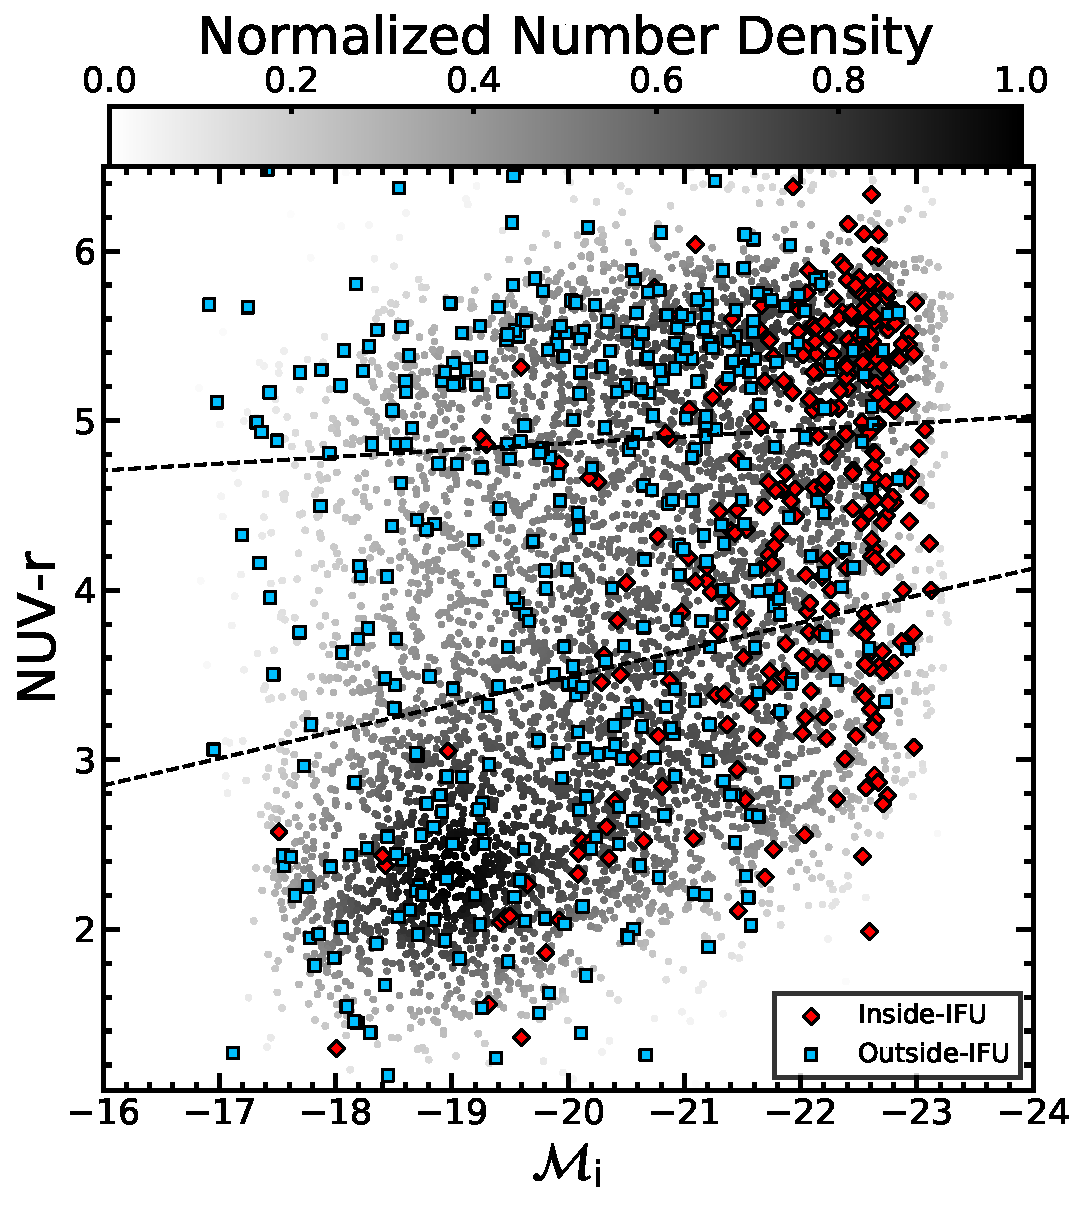
\includegraphics[width=\linewidth]{fig/color-mag.pdf}
\caption[]{Color-magnitude diagram for MaNGA galaxies ({\it colored circles}). The color of the symbol reflects the local density around each data point in this color-magnitude plane, as indicated by the color bar on the top. Inside and outside-IFU pairs are marked with {\it grey diamonds}. From top to bottom, the dashed lines divide the sample into red sequence, green valley, and blue cloud. The star-forming galaxy sample used in this paper are the galaxies below the lower dividing line.}
\label{fig:cmd}
\end{figure}
%%%%%%%%%%%%%%%%%%%%%%%%%%%%%%%%%%%%%%%%%%%%%%

MaNGA is an IFS survey at the Apache Point Observatory (APO) which used the SDSS (Sloan Digital Sky Survey) 2.5-meter telescope along with two dual-channel BOSS spectrographs \citep{Drory:2015}. MaNGA captures spectra through 17 integral field units (IFUs) with variable numbers of fibers; 19, 37, 61, 91, and 127 fibers covering 12.5\arcsec, 17.5\arcsec, 22.5\arcsec, 27.5\arcsec, and 32.5\arcsec on the sky respectively \citep{Law:2015}. MaNGA is an optical survey with a spectral coverage of 3600$-$10,300 \AA\ with a resolution of R $\sim$ 2000 and a PSF of 2.5\arcsec\ FWHM \citep{Bundy:2015}. 

The MaNGA survey targets galaxies from a subset of 41,154 galaxies from the NASA-Sloan Atlas (NSA v1\_0\_1; \url{http://www.nsatlas.org}) with a redshift range of 0.01 $< z <$ 0.15 and a luminosity range of -17.7 $<$ $\mathcal{M_{\rm i}}$ $<$ -24.0, where $\mathcal{M_{\rm i}}$ is the rest frame i-band magnitude within the survey's elliptical Petrosian apertures. MaNGA plans to cover 10,000 galaxies with a flat stellar mass distribution at two spatial coverages, 1.5 $R$/\reff\ and 2.5 $R$/\reff\ (where \reff\ is the radius which contains 50\% of the galaxy's total light). In this work we use the data from the internal data release, MPL-8, which covers 6142 unique galaxies. 

We classify galaxies in this survey as star forming galaxies using the color-magnitude diagram (CMD). We show the CMD for the MaNGA survey and our pair sample in Figure \ref{fig:cmd} along with demarcation lines which separate the blue cloud, red sequence, and green valley. We established the demarcation lines by collapsing the CMD to a color histogram for each of the three regions. We then varied the slopes between the regions until we found the slopes which best fit the data. These demarcation lines are;

\begin{equation}\label{eq:blue}
NUV-r = 3.1682 - 0.16 (\mathcal{M}_i+18)
\end{equation}
\begin{equation}\label{eq:red}
NUV-r = 4.7866 - 0.04 (\mathcal{M}_i+18)
\end{equation}

Where $NUV-r$ is the color from SDSS's k-corrected absolute magnitude and $\mathcal{M}_i$ is the i-band magnitude from the NSA catalog. We have checked the selected star forming galaxies on the BPT diagram \citep{Baldwin:1981} to confirm that AGN (active galactic nuclei) will have a minimal impact on our SFG sample.

On top of the color selection cuts, we require that all galaxies are in the Primary or Secondary MaNGA subsamples \citep{Wake:2017}, and that the stellar mass range of the galaxy sample is between \logm\ $=$ 9.0$-$11.5.

We build two different pair samples in this work; the inside-IFU sample which contains paired galaxies where both galaxies are covered by a single MaNGA IFU and the outside-IFU sample where a MaNGA target galaxy is coupled with another galaxy found outside of its MaNGA IFU. 

\subsection{Inside-IFU Sample}\label{sec:inside}

In our previous work, \citet{Fu:2018}, using the 2168 unique galaxies form DR14 \citep{Abolfathi:2018}, we showed that $\sim$5.7\% of the MaNGA observations have at least one companion galaxy within the field of view of the IFU. In this work we use a refined pair identification process which is also expanded for the most recent internal data release, MPL-8.

We identify potential paired galaxies by overlaying SDSS photometric objects over the MaNGA fields of view. We manually inspect each MaNGA field, removing photometric objects which are over-deblended galaxy fragments and adding any objects missed by the SDSS photometric catalog. At this stage the object catalog includes any foreground stars and foreground/background galaxies along with the potential paired galaxies. 

To select paired galaxies out of our object catalog, we inspect the spectra of each object. We use our own {\sc idl} based spectral fitting code, {\sc spfit}, to model the spectra from the MaNGA datacubes. {\sc spfit} simultaneously fits emission lines and the stellar continuum with the Levenberg-Marquardt nonlinear least-squares minimization algorithm \citep{Fu:2018}. Emission lines are parameterized as a Gauss-Hermite series and the stellar continuum is the sum of simple stellar populations (SSPs) convolved with the line-of-sight velocity distribution (LOSVD).

The spectra of the identified objects is extracted through a 1\arcsec\ circular aperture and fitted assuming the MaNGA target's redshift and then manually sorted into the following categories; ``good" galaxy spectra, broad-line AGN, foreground star, foreground/background galaxies, or poor S/N objects. The ``good" galaxy spectra are the objects whose spectra are well modeled by {\sc spfit} at the target galaxy's redshift, whether it is the target galaxy itself or a nearby companion galaxy. This means that the companion galaxy can be within $\pm$3000 km s$^{-1}$ of the MaNGA target. We found 6573 ``good" objects, 57 broad-line AGN, 836 foreground stars, 319 foreground/background galaxies, and 1546 objects with poor S/N. 

From the 6573 galaxies with good spectra, 404 of the MaNGA IFUs have multiple objects within the IFU. We further restrict the sample by setting a relative velocity cut of $\Delta v$ $<$ 500 km s$^{-1}$ to remove projected companions. Given redshift range of the MaNGA sample and the size of MaNGA's IFUs, the maximum projected separation for a companion galaxy in the IFU is $\sim$40 kpc. Again, the galaxy sample is also restricted to galaxies with a stellar mass range of \logm\ $=$ 9.0$-$11.5 and galaxies in the Primary or Secondary MaNGA subsamples. We also require that the galaxies are classified as star forming by the CMD diagram. These requirements reduce our sample down to 87 star forming galaxies (SFGs). 

Several of the target galaxies in our sample have multiple companions. From the whole set of 404 IFUs, there are 327 pairs, 67 triplets, 7 quadruplets, and 1 quintuplet. 

\subsection{Outside-IFU Sample}\label{sec:outside}

We supplement the inside-IFU sample with a set of pairs identified outside of the field of view of the MaNGA IFU. We select these outside-IFU pairs from the NSA catalog. We search for these external pairs by selecting objects with a projected separation from the MaNGA targets of $r_p$ $<$ 50 kpc using the MaNGA target's redshift. We further use a relative velocity cut of $\Delta v$ $<$ 500 km s$^{-1}$ to remove projected galaxies from the selection. 

From the NSA catalog's 641,409 galaxies, we find 492 galaxies which are paired to MaNGA targets. MaNGA targets which have both an inside-IFU and an outside-IFU pair are left to the inside-IFU sample. After restricting the sample to SFGs, we have another 133 MaNGA targets with paired galaxies outside of the IFU. This give use a total of 220 MaNGA targets in our pair sample.

\subsection{Control Sample}\label{sec:control}

To show how the population of galaxy pairs differs from isolated galaxies, we will compare our pair sample to a sample of isolated galaxies in the MaNGA survey. We build this control sample from the MaNGA target galaxies which have no spectroscopic companions within $r_p$ $<$ 50 kpc and $\Delta v$ $<$ 500 km s$^{-1}$ either inside or outside of the IFU. This gives us a control sample of 1891 star forming control galaxies. 

It has been shown that the SFR in galaxies is dependent on both the stellar mass and the redshift of the galaxies \citep{Noeske:2007}. We will compare our interacting galaxies with isolated galaxies of a similar stellar mass and redshift, to account for these other dependencies. To do this, we will use two different methods of pair - control comparison. 

In the first method, we only control for the stellar mass between the pairs and controls. We split both the pair and control samples into five evenly spaced stellar mass bins over the range, \logm\ $=$ 9.0$-$11.5. The pairs are then compared to their respective controls within each stellar mass bins. While the redshift in not constrained in this method, we will show in Section \ref{sec:mass-bin} that this method is sufficient to reveal the merger induced star formation. 


In the second method, we wish to account for both stellar mass and redshift. To do this we select a subsample of 20 control galaxies for each paired galaxy. We first select all of the control galaxies which are within a 0.1 dex stellar mass limit and within the same MaNGA subsample (e.g. Primary or Secondary) as the paired galaxy. Since the MaNGA sample has a tight distribution in stellar mass and redshift, the stellar mass and MaNGA subsample restriction effectively sets a $z$ $\lesssim$ $\sim$0.025 redshift cut. 

Setting the above requirements, most paired galaxies will find between 20$-$100 control galaxies. Since we want each paired galaxy to be treated in a similar manner, we will down-select the total number of acquired control galaxies down to 20 controls randomly. In the cases where a paired galaxy does not initially acquire 20 control galaxies we iteratively expand the stellar mass limit by 0.1 dex until at least 20 control galaxies are found. A small set of paired galaxies required extra iterations to find 20 controls; 8 needed an extra iteration, 1 needed two extra iterations, and 1 needed three iterations.

While the first method is less sophisticated in comparison to the second method, we will see in Section \ref{sec:results} that the first method is sufficient to see the central enhancement to the star formation rate and the mass independence of the star formation enhancement.

%%%%%%%%%%%%%%%%%%%%%%%%%%%%%%%%%%%%%%%%%%%%%%%%%%%%
\section{Radial Profiles of Star Formation}\label{sec:analysis}

\subsection{Specific Star Formation Rate}

%%% SPFIT
We use our spectral fitting code, {\sc spfit}, to get measurements of emission line fluxes, equivalent widths, velocities, and velocity dispersions of 19 emission lines and measurements of stellar masses, ages, [Fe/H], and the kinematics of the stellar populations. 

%%% Reddening
We correct the emission lines for reddening using the extinction curve from \citet{Cardelli:1989} with updated coefficients from \citet{ODonnell:1994}. The extinction in parameterized as R$_V$ $\equiv$ A$_V$/E(B$-$V) $=$ 3.1, where we estimate the value of the V-band extinction, A$_V$, by comparing the H$\alpha$/H$\beta$ ratio to the expected value of 2.85 for case-B recombination. 

\begin{equation}
A_V = 6.78\ {\rm log} \left[(H\alpha/H\beta)/2.85 \right]
\end{equation}

We measure the SFR from the extinction corrected H$\alpha$ luminosity, L$_{{\rm H}\alpha}$, calculated from the H$\alpha$ flux.  We use the SFR formula, Equation \ref{eq:sfr}, from \citet{Murphy:2011} which uses a Kroupa IMF, Solar metallicity, a constant SFR at an age of 100 Myr, and Case-B recombination. 

\begin{equation}\label{eq:sfr}
\frac{\rm{SFR}}{M_{\odot} \, \rm{yr^{-1}}} = \frac{{\rm L}_{H\alpha}}{1.86 \times 10^{41}\, \rm{erg\,s}^{-1}}
\end{equation}

Since the stellar mass of a galaxy is not uniformly distributed within the galaxy, we normalize the SFR by the local stellar mass, $M_*$, giving us the specific star formation rate (sSFR). The local stellar masses used here is the stellar mass calculated by {\sc SPFIT}'s fit to the stellar continuum within each spaxel (spatial pixel).

\begin{equation}
{\rm sSFR} = \frac{\rm SFR}{M^*}
\end{equation}

This will allow us to compare regions to high mass surface density to regions of low mass surface density. 

We check the results of the radial profiles of this sSFR against the radial profiles of \ewha\ and find that they are in good agreement. \ewha\ is an observable while our measurement of the sSFR is dependent on both the H$\alpha$ luminosity and {\sc spfit}'s calculation of the stellar mass, so this check helps confirm the quality of our sSFR measurement.

It has been shown that hot low mass evolved stars (HOLMES) in retired galaxies can mimic H\,{\sc ii} regions and AGN on the BPT diagram \citep{Stasinska:2008}. To mask retired spaxels, we implement a H$\alpha$ equivalent width (EW) cut of \ewha\ $>$ 3\AA\ \citep{Cid-Fernandes:2011}. 

%%%%%%%%%%%%%%%%%%%%%%%%%%%%%%%%%%%%%%%%%%%%%%%%%%%%
\subsection{Radial Profiles}\label{sec:radial}

%%%%%%%%%%%%%%%%%%%%%%%%%%%%%%%%%%%%%%%%%%%%%%
\begin{figure*}
\centering
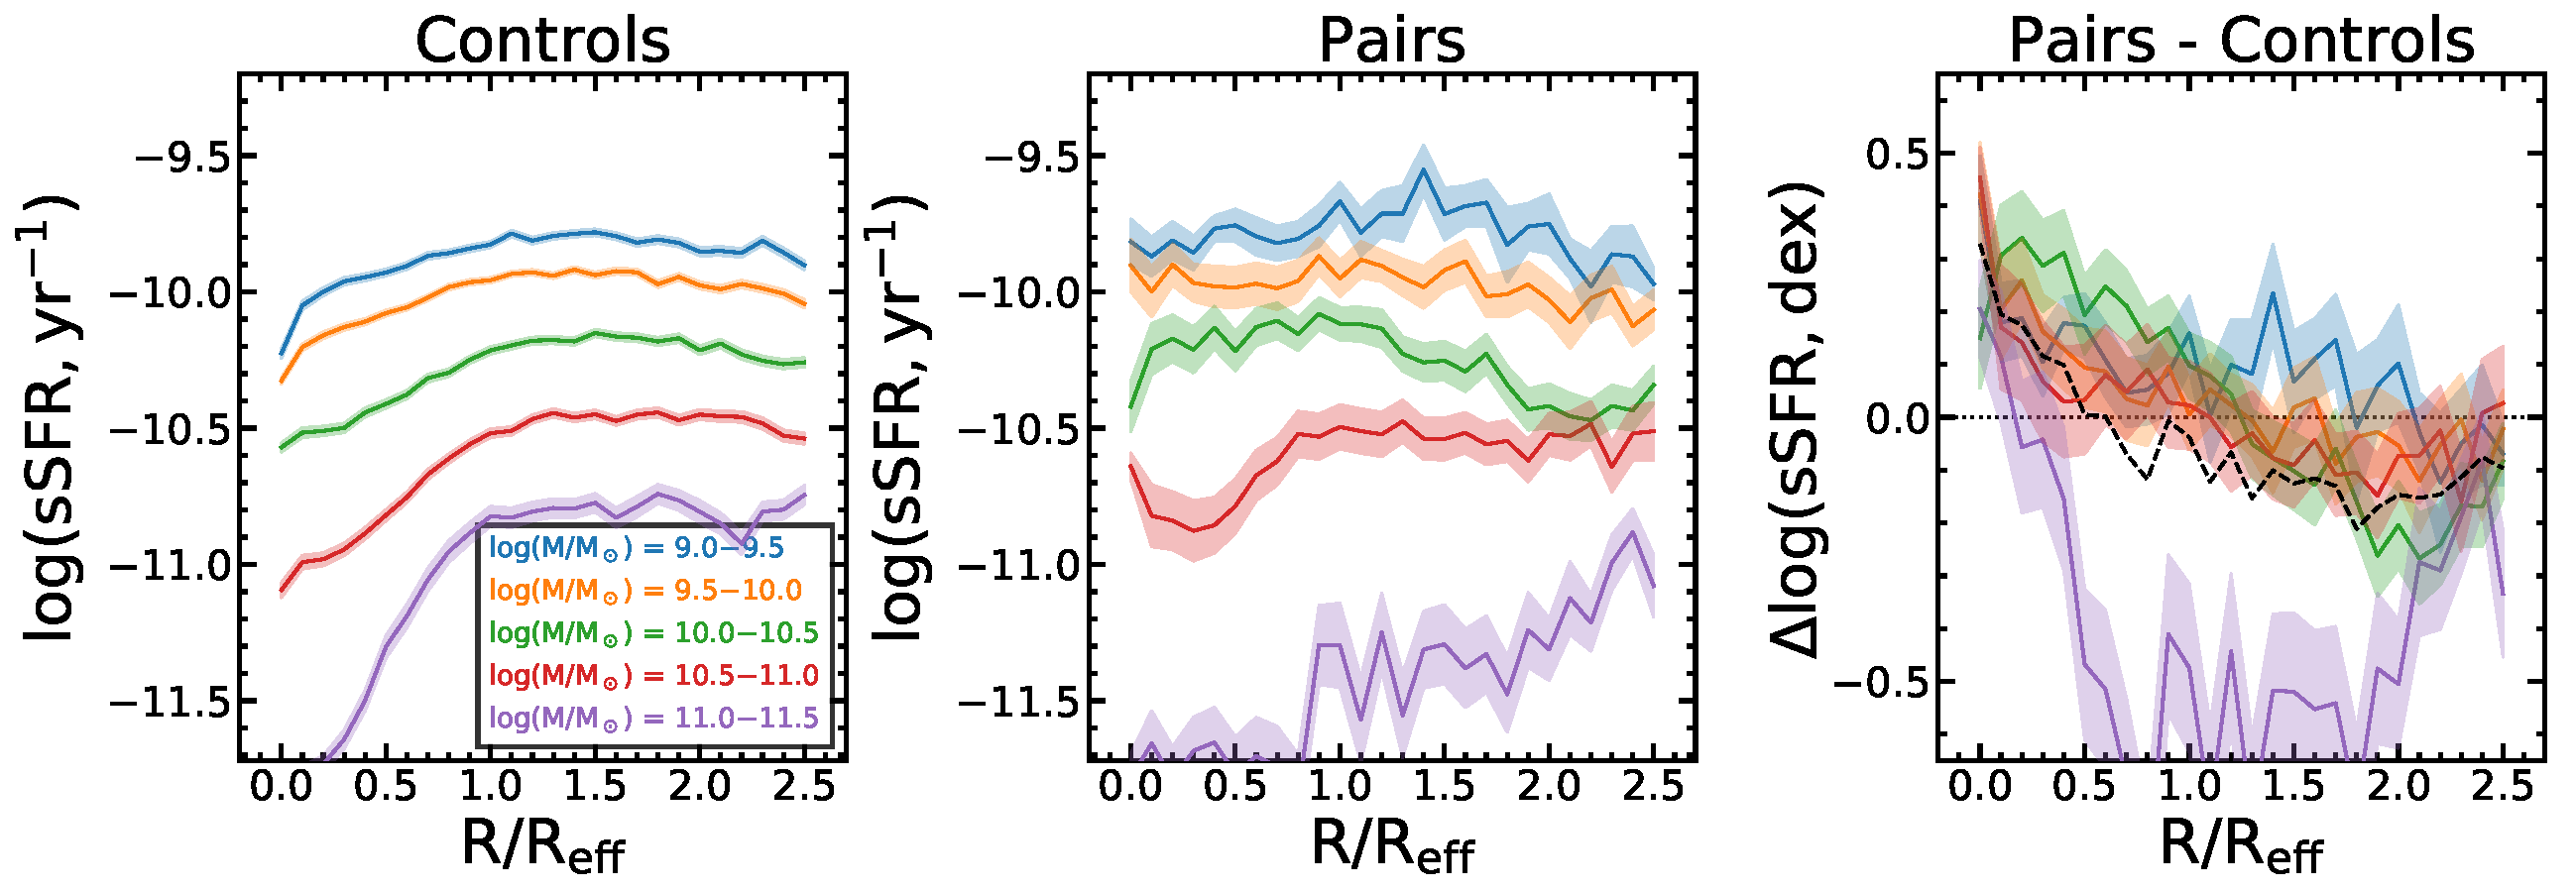
\includegraphics[width=\linewidth]{fig/ssfr_comb.pdf}
\caption[]{The log(sSFR) as a function of galactocentric radius for control galaxies (\textbf{Left}) and galaxy pairs (\textbf{Middle}). The difference between the profiles of the paired galaxies and the control galaxies are shown in the \textbf{Right} panel. The dashed black profile represents the mean of the difference profiles). The colors of the profiles represent the mass range of the selected galaxies and the highlighted region around the profiles represent the standard error of the mean of the data at the given radius interval.}
\label{fig:ssfr_prof}
\end{figure*}
%%%%%%%%%%%%%%%%%%%%%%%%%%%%%%%%%%%%%%%%%%%%%%

In order to spatially characterize the star formation in the paired galaxies we build radial profiles of sSFR. First, the geometry of the galaxies needs to be defined. Specifically we will need position angle, inclination angle, and the effective radius of each of the MaNGA targets. We use the $r$-band elliptical Petrosian apertures from the NSA catalog and the $r$-band S\'ersic apertures from \citet{Simard:2011} to define the geometries of the galaxies. 

The NSA catalog has complete coverage over the MaNGA sample (since MaNGA selects its targets from this catalog); however, it tends to fail to properly fit paired galaxies with close on-sky separations. We found that the apertures from \citet{Simard:2011} work better for these close paired galaxies; however, the catalog does not completely cover the MaNGA sample. We use the NSA catalog for the outside-IFU pair sample because they are well separated on the sky. The \citet{Simard:2011} catalog is used for the inside-IFU sample. If the paired galaxy is not covered by \citet{Simard:2011}, we use the ellipse from the NSA catalog. 

We fit the geometry with apertures from both catalog when available. When using the first method of pair-control comparison, where pairs and controls are grouped into stellar mass bins, we fit the control galaxies with the NSA apertures. When making the comparison with the second method, paired galaxies fitted with the NSA aperture are compared against controls fitted with the NSA aperture and paired galaxies fitted with the \citet{Simard:2011} apertures are compared against controls fitted with the \citet{Simard:2011} apertures. 

We compared the magnitudes extracted from the two apertures for the control galaxies and found that they are in close agreement. This means that the geometries between the two surveys must be in close agreement and the profiles of a galaxy fitted with a NSA aperture can be confidently compared against a galaxy fitted with an aperture from \citet{Simard:2011}. 

We calculate the inclination angle, {\it i}, of the galaxies using the major-to-minor axis ratios from the elliptical apertures;

\begin{equation}
{\rm cos^2}(i) = \frac{(b/a)^2 - q^2}{1 - q^2}
\end{equation}

Where $b/a$ is the major-to-minor axis ratio and $q$ is the intrinsic oblateness. We use the empirically determined oblateness of $q = 0.13$, from \citet{Giovanelli:1994}.

The inclination angle, along with the galaxy's position angle, is used to deproject the geometries of the galaxies. We use the 50\% half light radius (i.e. the effective radius, \reff) to scale the sizes of the galaxies. Doing this will allow us to compare galaxies of different sizes against each other.

Once the geometry of the galaxies are set, we can build the radial profiles. The spaxels are binned into radius increments of 0.1 R/\reff\ from 0.0$-$2.5 R/\reff. Within each radius bin we take the median of the specific star formation rate. The profiles' errors are the standard error of the mean of the data within each radius bin. We create one of these individual averaged radial profiles for every MaNGA galaxy. 

We use our catalog of photometric objects and the \citet{Simard:2011} catalog to mask foreground/background objects within the MaNGA IFUs which may contaminate the data. Objects in our photometric catalog are masked out with a 2\arcsec\ circular aperture and the galaxies from \citet{Simard:2011} are masked out with a 2.0 R/\reff\ elliptical aperture, using the r-band S\'ersic apertures from the catalog. This gives us an individual radial profile of the sSFR for all paired and control galaxies.


%%%%%%%%%%%%%%%%%%%%%%%%%%%%%%%%%%%%%%%%%%%%%%%%%%%%
\section{Results}\label{sec:results}

\subsection{Star Formation Enhancement}

With individual log(sSFR) profiles built for each MaNGA galaxy, we now use two different methods to compare the profiles of paired galaxies against the profiles of control galaxies. The first method, in Section \ref{sec:mass-bin}, paired galaxies are compared to control galaxies within evenly spaced stellar mass-bins. In the second method, in Section \ref{sec:tailored}, paired galaxies are compared to a subset of 20 control galaxies which have a similar stellar mass and redshift. 

\subsubsection{Mass-Binned Difference Profiles}\label{sec:mass-bin}

In the first method, paired and control galaxies are grouped into five evenly spaced stellar mass bins between \logm\ $=$ 9.0$-$11.5. Within each stellar mass bin, we create a median profile of log(sSFR) as a function of galactocentric radius for both paired and control galaxies. The control profiles are constructed using all available control galaxies within each mass bin. The error associated with the profile is the standard error of mean of the data at each radius bin. We show these ``stacked" profiles for control galaxies in the left hand panel of Figure \ref{fig:ssfr_prof} and the stacked profiles for paired galaxies in the middle panel of Figure \ref{fig:ssfr_prof}.

Once the stacked profiles are made, we take the difference between the stacked profiles of the paired galaxies and the control galaxies, pair - control, in log space (this means that the profiles really represents a ratio between the pairs and controls in linear space). This gives us difference profile, $\Delta$log(sSFR), which shows us where the sSFR is enhanced or suppressed (shown in the right hand panel of Figure \ref{fig:ssfr_prof}). 

The dashed regions of the profiles in Figure \ref{fig:ssfr_prof} represent regions which have been ``trimmed" due to a low percent of data coverage in the region. A radial bin is trimmed if less than 70\% of the galaxies in that bin have data. There are a few reasons why galaxy's profile may not have data points at a given radial bin. First, the MaNGA IFU may not cover the radius range; only $\sim$37\% of MaNGA galaxies are covered out to 2.5 $R$/\reff. This radial coverage limitation primarily affect the lower mass galaxies in the \logm\ $=$ 9.0$-$9.5. Second, foreground and background objects have been masked out which can create gaps in the data of an individual galaxies profile. This case does not significantly affect the stacked profiles here since the masked out regions will be spread out across the whole radius range. Third, retired regions within galaxies have been masked out with the \ewha\ $\ge$ 3\AA\ cut. It is well known that high mass galaxies tend to be passive (as seen in our CMD diagram in Figure \ref{fig:cmd}). As a consequence, the highest mass galaxies in our sample (\logm\ $=$ 11.0$-$11.5) have much of their profiles trimmed due to absence of star forming spaxels. 

This method has the benefit of a high S/N control profile since each mass bin will have hundreds of control galaxies while the median control profiles of the second method will only have 20 controls. On the other hand, this method only controls for a single galaxy parameter, stellar mass. Further the profiles can only be studied as a function of stellar mass so we are unable to study the profiles as a function of projected separation or mass ratio. 

Between the median profiles of the control galaxies and paired galaxies, we can see that the paired profiles are flattened in their centers in comparison to the control profiles. The paired profiles are centrally enhanced by $\sim$0.25 $\pm$ 0.1 dex. This enhancement linearly falls to zero around 1.0 $R$/\reff. In the disks the profiles feature a weak suppression to the sSFR of 0.05$-$0.1 dex. 

The sSFR in the pair sample shows no dependence on their stellar mass. The profiles from all of the mass ranges fall within $\sim$0.2 of the median profile. This means that low mass galaxies are enhanced at the same level as high mass galaxies. It is also notable that while this method of pair-control comparison is not rigorous as the next method, the central star formation enhancement is clearly present at all stellar masses.

The higher rate of star formation within interacting galaxies will mean that the stellar mass in the interacting galaxies will grow at a faster rate compared to secular mass growth. The fractional mass growth rate is simply the difference between the sSFR profiles of the paired and control galaxies (pairs - controls) multiplied by at timescale. We chose a timescale of 1 Gyr as an order of magnitude estimate of the interaction event \citep{Boylan-Kolchin:2008}, though the actual timescale of the merger induced starburst is likely somewhat shorter ($\sim$0.4 Gyr; \citet{Feng:2019}). 

Since the $\Delta$log(sSFR) is independent of galaxy mass, the fractional mass change will depend on the stellar mass of the paired galaxy. Low mass galaxies, \logm\ $=$ 9.0$-$9.5, experience a fractional mass change of $\Delta M_{\rm merger}$/$M_{\rm total}$ $=$ 0.06 (6\%) while massive galaxies, \logm\ $=$ 11.0$-$11.5, experience a fractional mass change of $\Delta M_{\rm merger}$/$M_{\rm total}$ $=$ 0.005 (0.5\%). This show that the merger induced mass growth is greatest in low mass galaxies. Further, the merger induced mass growth is restricted to the centers of the paired galaxies which will result in galaxies which have more prominent bulges in their centers. 

\subsubsection{Tailored-Controls Difference Profiles}\label{sec:tailored}

In the second method, we match each paired galaxy to a set of 20 control galaxies of similar stellar masses and redshifts, as described in Section \ref{sec:control}. We take the individual azimuthally averaged profiles of the selected control galaxies and take the median value of the profiles at each radius bin to produce the average profile of the control galaxies. 

% Is this necessary
%The error of the profile is the standard error of the mean of the individual profiles. We also take into account the error associated with the random selection of controls using a bootstrapping method to quantify the variation in the values of the stacked profiles over 1000 iterations. We estimate that this random selection contributes an error of about 0.1 dex.

Once the average profile of the control galaxies is made, we take the difference between the paired galaxy's profile and the average control profile in log space. We do this process for each of the 220 paired galaxies. 

The difference profiles at this stage have now been controlled for stellar mass and redshift. We can freely stack these difference profiles to study their dependence on other parameter like the mass ratio and projected separation. We split the individual difference profiles into five evenly spaced stellar mass bins between \logm\ $=$ 9.0$-$11.5 and stack the difference profiles within each mass bin. This gives us five difference profiles covering five different stellar mass ranges shown in the left hand panel of Figure \ref{fig:ssfr_mass}. The errors of the stacked profiles are the standard error of the mean of the difference profiles within each bin.

The difference profiles are shown to be centrally enhanced by $\sim$0.25 $\pm$ 0.1 dex. The enhancement falls to zero around 1.0 \reff\ and is slightly suppressed in their disks by $\sim$0.1 dex. While all of the other paired galaxies show a sSFR suppression in their disks, the profiles of the pairs in the stellar mass range of \logm\ $=$ 9.0$-$9.5 show an enhancement in their disks of $\sim$0.1$-$0.2 $\pm$ 0.1 dex. 

The profiles are largely consistent with the results of the previous mass binning method. The profiles of this method have less scatter as a result of how the paired are more closely matched in stellar mass and redshift. This method also has the added benefit that the profiles can be separated by parameters other than stellar mass. We will discuss how these profiles behave as a function of the mass ratio and projected separation in the following sections. 

We can also inspect the star formation enhancement within individual paired galaxies. We extract the $\Delta$log(sSFR) from the individual difference profiles. We extract the value of $\Delta$log(sSFR) from the inner 0.5 $R$/\reff\ of the paired galaxies and take the mean value of the $\Delta$log(sSFR) within the aperture. We depict the central $\Delta$log(sSFR) as a function of stellar mass in the right hand panel of Figure \ref{fig:ssfr_mass}. The mass independence can be clearly seen here as the paired galaxies within each stellar mass bin fall within 0.1 dex of the 0.2 dex $\Delta$log(sSFR) median. 

Between the two different pair-control comparison methods, we conclude that the $\Delta$log(sSFR) is independent of the paired galaxies' stellar mass. Low mass galaxies are having their sSFR enhanced at a similar rate as high mass galaxies. 

%\subsection{Future Mass Growth}

%The higher rate of star formation within interacting galaxies will mean that the stellar mass in the interacting galaxies will grow at a faster rate compared to secular mass growth. The question is whether or not the advanced mass growth rate is significant. 

%To estimate the enhanced mass growth rate due to merger induced star formation, we will assume a constant star formation rate over a given timescale, $\tau$. A specific star formation rate is already a representation of the fractional mass growth every year, so the merger induced mass growth is simply;

%\begin{equation}
%\frac{\Delta M_{merger}}{M_{total}} = \left({\rm sSFR}_{\rm pair} - {\rm sSFR}_{\rm control}\right) * \tau
%\end{equation}

%For this estimation we use a timescale of 1 Gyr, which is the order of the typical timescale between the passage of the first and second pericenters in dark-matter simulations \citep{Boylan-Kolchin:2008}. The actual timescale for star formation enhancement is likely shorter; however, we will use the 1 Gyr value as an order of magnitude estimate. 

%To get the difference in sSFR between the pairs and controls, we fit a gaussian to the difference profiles split by stellar mass. We then add the modeled difference profile to the stacked control profile in the same mass range in log space. We then take the difference between the profiles in linear space and multiply the difference by the 1 Gyr timescale. 

%We show the mass growth rate profile for each of the four mass ranges in Figure \ref{fig:mass_gain_sum}. The mass growth rate is largely restricted to the centers of the galaxies and falls to zero around 1.0 R/\reff, following profile of the $\Delta$log(sSFR). The mass growth rate is strongly dependent on the stellar mass of the paired galaxies. 

%The fractional mass change is greatest in the less massive galaxies, $\Delta$M$_{merger}$/M$_{total}$ $=$ 0.06 (6\%), while it is less substantial is the more massive galaxies, $\Delta$M$_{merger}$/M$_{total}$ $=$ 0.005 (0.5\%). This is unsurprising as the $\Delta$log(sSFR) profiles were independent of the galaxies' total stellar mass. 

%In the context of galaxy evolution, where less massive galaxies merge to form larger galaxies, the merger induced star formation contributes a significant amount of stellar mass on top of the stellar mass contribution from the mixing of the two galaxies. Further, the merger induced mass growth is restricted to the centers of the paired galaxies which will result in galaxies which have more prominent bulges in their centers.  

%%%%%%%%%%%%%%%%%%%%%%%%%%%%%%%%%%%%%%%%%%%%%%
\begin{figure*}
\centering
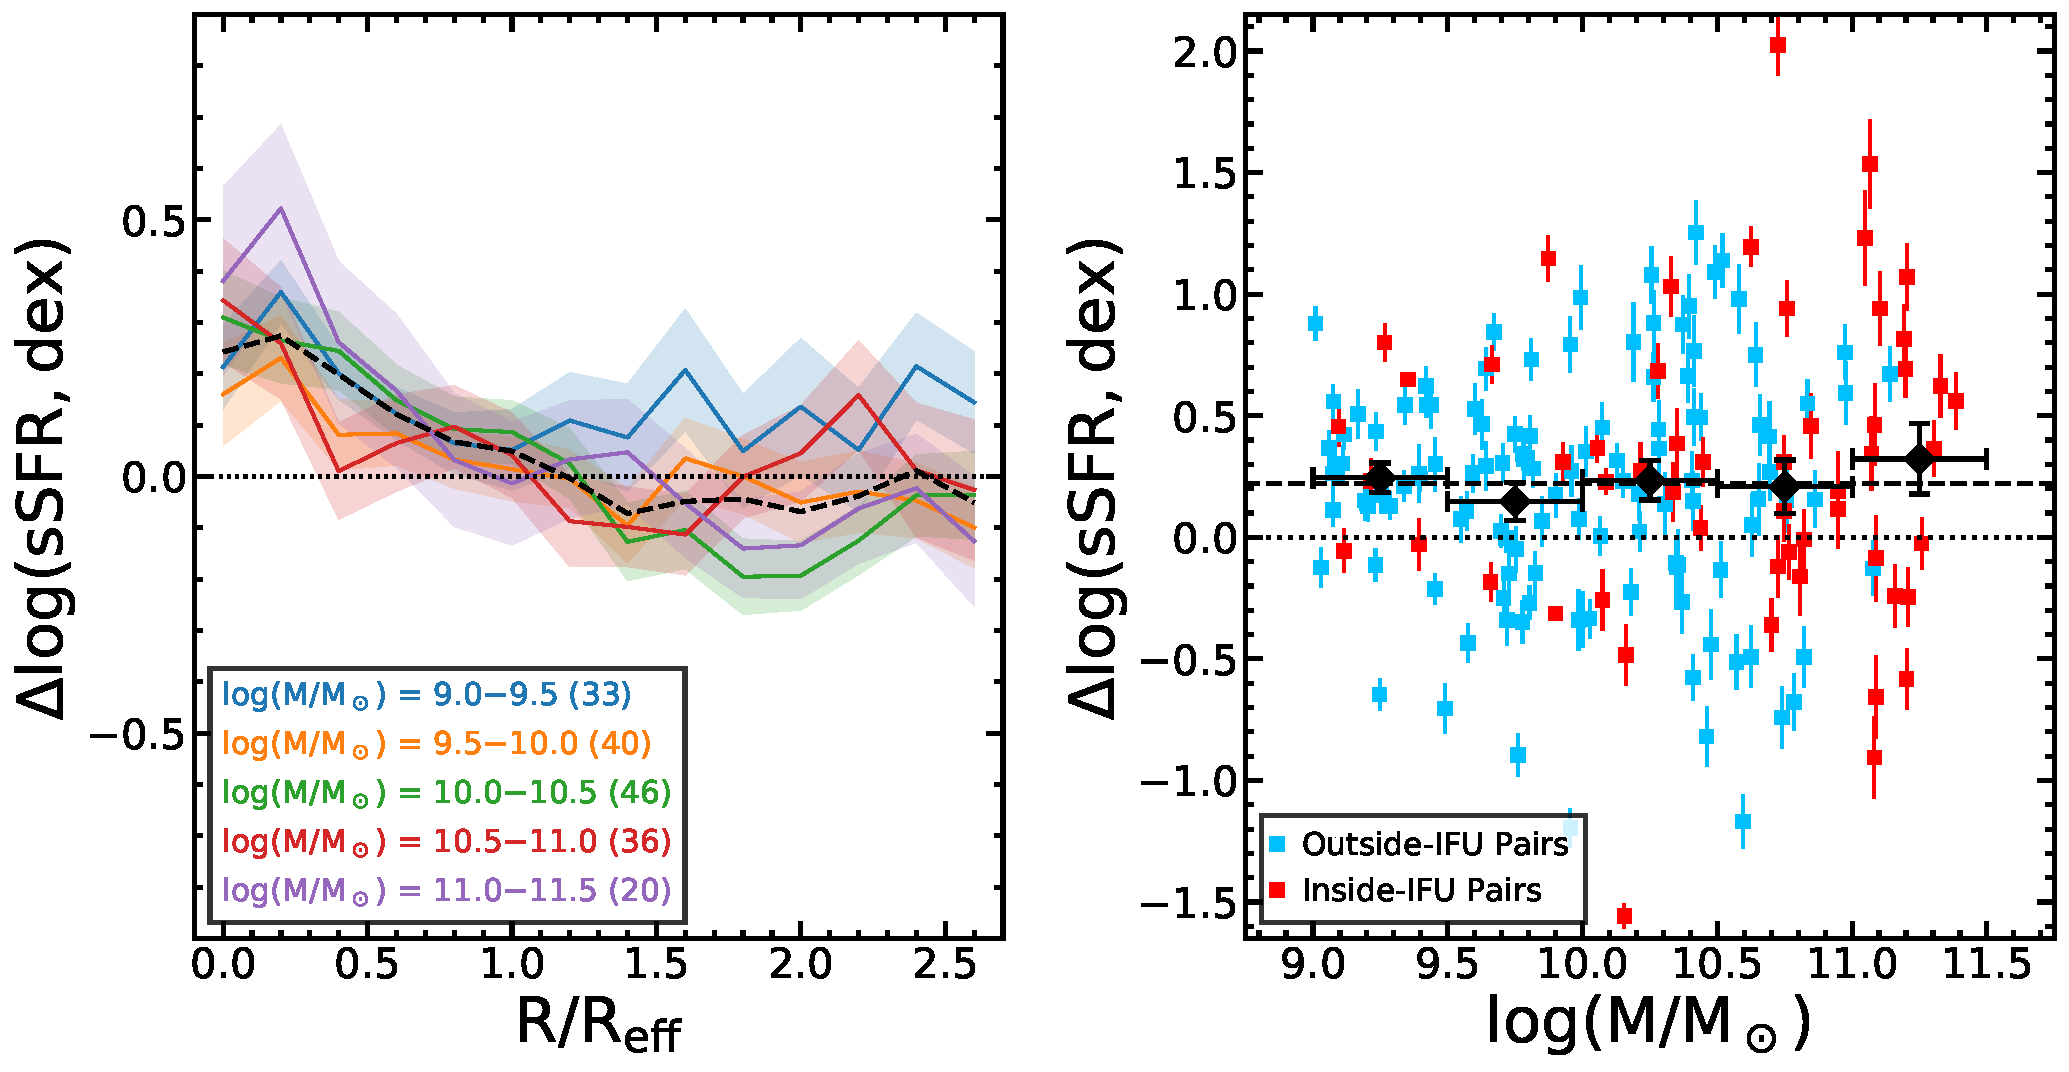
\includegraphics[width=\linewidth]{fig/ssfr_mass.pdf}
\caption[]{The \textbf{Left} panel shows the $\Delta$log(sSFR) profiles where the difference profiles are constructed from the difference between the paired galaxy profiles and a set of 20 control galaxies. The profiles are split into four different stellar mass bins and the highlighted region about the profiles represent the standard error of mean of the profile. The black dashed line represents the mean profile between the four difference mass ranges. In the \textbf{Right} panel the nuclear $\Delta$log(sSFR) are shown. The black squares are the mean values within a stellar mass bin (where the size of the bins are shown the the horizontal error bars). The vertical error bars on the black squares represent the standard deviation within the bin. The horizontal, dashed black line represents the median central enhancement of the pair sample. Galaxies in the outside-IFU (Blue) and inside-IFU (Red) samples are separately depicted.}
\label{fig:ssfr_mass}
\end{figure*}
%%%%%%%%%%%%%%%%%%%%%%%%%%%%%%%%%%%%%%%%%%%%%%

\subsection{Dependency on Mass Ratio}
While the total stellar mass of the galaxies has no effect on the merger induced star formation, the mass ratio between the paired galaxies does. The mass ratio here is calculated as the difference between stellar masses contained within the 50\% half light radius, 

\begin{equation}
\Delta {\rm log}(M) = {\rm log}(M_{\rm target}) - {\rm log}(M_{\rm comp}) 
\end{equation}

Where $M_{\rm target}$ is the stellar mass of the MaNGA target galaxy and $M_{\rm comp}$ is the stellar mass of the companion galaxy. 

For the outside-IFU sample we use the stellar masses calculated from the r-band elliptical Petrosian apertures from the NSA catalog. Most of the companion galaxies in the inside-IFU sample are not covered by either the NSA catalog or \citet{Simard:2011}. Because of this, the inside-IFU galaxies are left out of this analysis.

In the Top row of Figure \ref{fig:ssfr_dmsep} we see that the sSFR enhancement is strongest in galaxies close to a 1:1 mass ratio, $\Delta$log($M$) $=$ 0.0. These galaxies feature a central enhancement of $\sim$0.3 dex which is 0.1 dex higher than the average central enhancement of the whole sample. This enhancement falls with wider mass ratio; however, pairs with large differences in stellar mass still feature substantial levels of star formation enhancement, 0.15$-$0.20 dex at mass ratios of $|\Delta$log($M$)$|$ $=$ 1.0.

We also use the mass ratio to explore how the merger induced tidal torques affect paired galaxies with large mass ratios, $|\Delta$log($M$)$|$ > 0.5. We use the mass ratio to separate the massive central galaxy from satellite galaxies. A paired galaxy with a positive mass ratio is the more massive galaxy of the pair while a paired galaxy with negative mass ratio is the less massive galaxy. We see that the less massive galaxy of a pair show a higher level of sSFR enhancement, by $\sim$0.1 dex, with respect to the more massive galaxy. This shows us that satellite galaxies may be more susceptible to tidal interactions than the central galaxies in the pair system. 

In previous studies it was noted that the enhancement to the SFR is strongest in galaxy pairs with small mass ratios \citet{Ellison:2008}. We see the same effect; however, we have also found that galaxy pairs with large mass ratios still show a substantial level of sSFR enhancement. It has been a convention to split galaxy pairs in major mergers, $|$log($M$)$|$ $\le$ 0.5, and minor mergers 0.5 $<$ $|$log($M$)$|$ $\le$ 1.0. In this work, we can see that the mass ratio range used in galaxy pair studies could be widened to at least $|$log($M$)$|$ $\le$ 1.5 so that larger pair samples can be constructed.  

Further, within these galaxy pairs with wide mass ratios we see that the less massive galaxy in the pair ($\Delta$log($M$) $<$ 0) shows higher levels of sSFR enhancement. This implies that satellite galaxies are more affected by interaction induced star formation than the central galaxy. 

\subsection{Dependency on Projected Separation}\label{sec:sep}

We also look at the level of sSFR enhancement as a function of the projected separation between the two galaxies in the bottom row of Figure \ref{fig:ssfr_dmsep}. The $\Delta$log(sSFR) profiles show a clear gradient with the projected separation where close galaxy pairs show higher levels of sSFR enhancement compared to pairs with wide separations. The profiles in the galaxy pairs in the separation range, $r_{\rm p}$ $=$ 0.0$-$12.5, are generally $\sim$0.1 dex above the median and the profiles of the galaxy pairs in the separation range, $r_{\rm p}$ $=$ 37.5$-$50.0, are generally $\sim$0.1 dex below the median. 

This effect can be seen most clearly in the scatter plot of the central $\Delta$log(sSFR) enhancement as a function of projected separation. The level of the enhancement gradually increases with closer separation from 50 kpc to 10 kpc. While $\Delta$log(sSFR) falls at higher separations, there is still a substantial level of enhancement between 40 and 50 kpc, $\sim$0.1$-$0.2 dex. Within 15 kpc, the $\Delta$log(sSFR) enhancement jumps to 0.3$-$0.4 dex. 

The sSFR enhancement increasing with closer projected separations is to be expected and has been shown in previous studies \citep{Li:2008, Ellison:2008, Scudder:2012, Patton:2013}. The passage of the first pericenter is predicted to trigger a burst of star formation which falls as the two galaxies separate \citep{Scudder:2012}. The sSFR enhancement in our sample persists out to 50 kpc. \citet{Patton:2013} showed that the burst of star formation can persist out to 150 kpc. 

For galaxies with separations of $r_{\rm p}$ $<$ 5 kpc and $r_{\rm p}$ $=$ 30$-$35 kpc we find a $\Delta$log(sSFR) of zero. For the $r_{\rm p}$ $<$ 5 kpc galaxies, about half of the pairs show signs of tidal features while the others do not. The pairs without the tidal features may be approaching their first pericenter, meaning that the merger-induced gas-inflows have not been triggered yet. The dips in $\Delta$log(sSFR) may also just be due to statistical error from the relatively limited sample size.  

%%%%%%%%%%%%%%%%%%%%%%%%%%%%%%%%%%%%%%%%%%%%%%%%%%%%
\section{Discussion}\label{sec:disc}
%%%%%%%%%%%%%%%%%%%%%%%%%%%%%%%%%%%%%%%%%%%%%%
%\begin{figure}
%\centering
%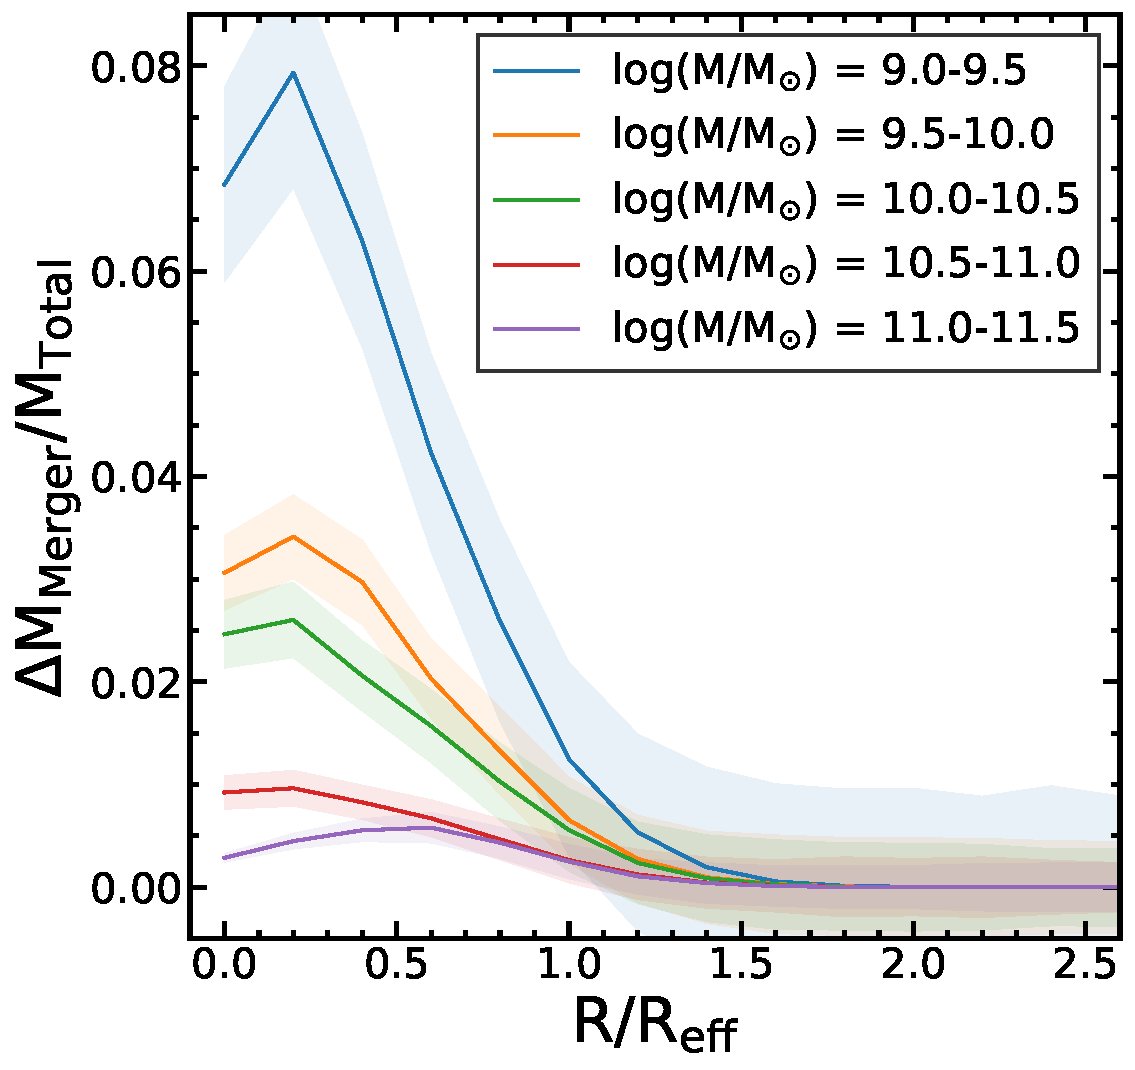
\includegraphics[width=3in]{fig/mass_gain.pdf}
%\caption[The fractional mass gain due to merger induced star formation.]{The fractional mass growth due to merger induced star formation over 1 Gyr. The highlighted region represents the propagated standard errors of the mean of the stacked log(sSFR) profiles. }
%\label{fig:mass_gain_sum}
%\end{figure}
%%%%%%%%%%%%%%%%%%%%%%%%%%%%%%%%%%%%%%%%%%%%%%

%%%%%%%%%%%%%%%%%%%%%%%%%%%%%%%%%%%%%%%%%%%%%%
\begin{figure*}
\centering
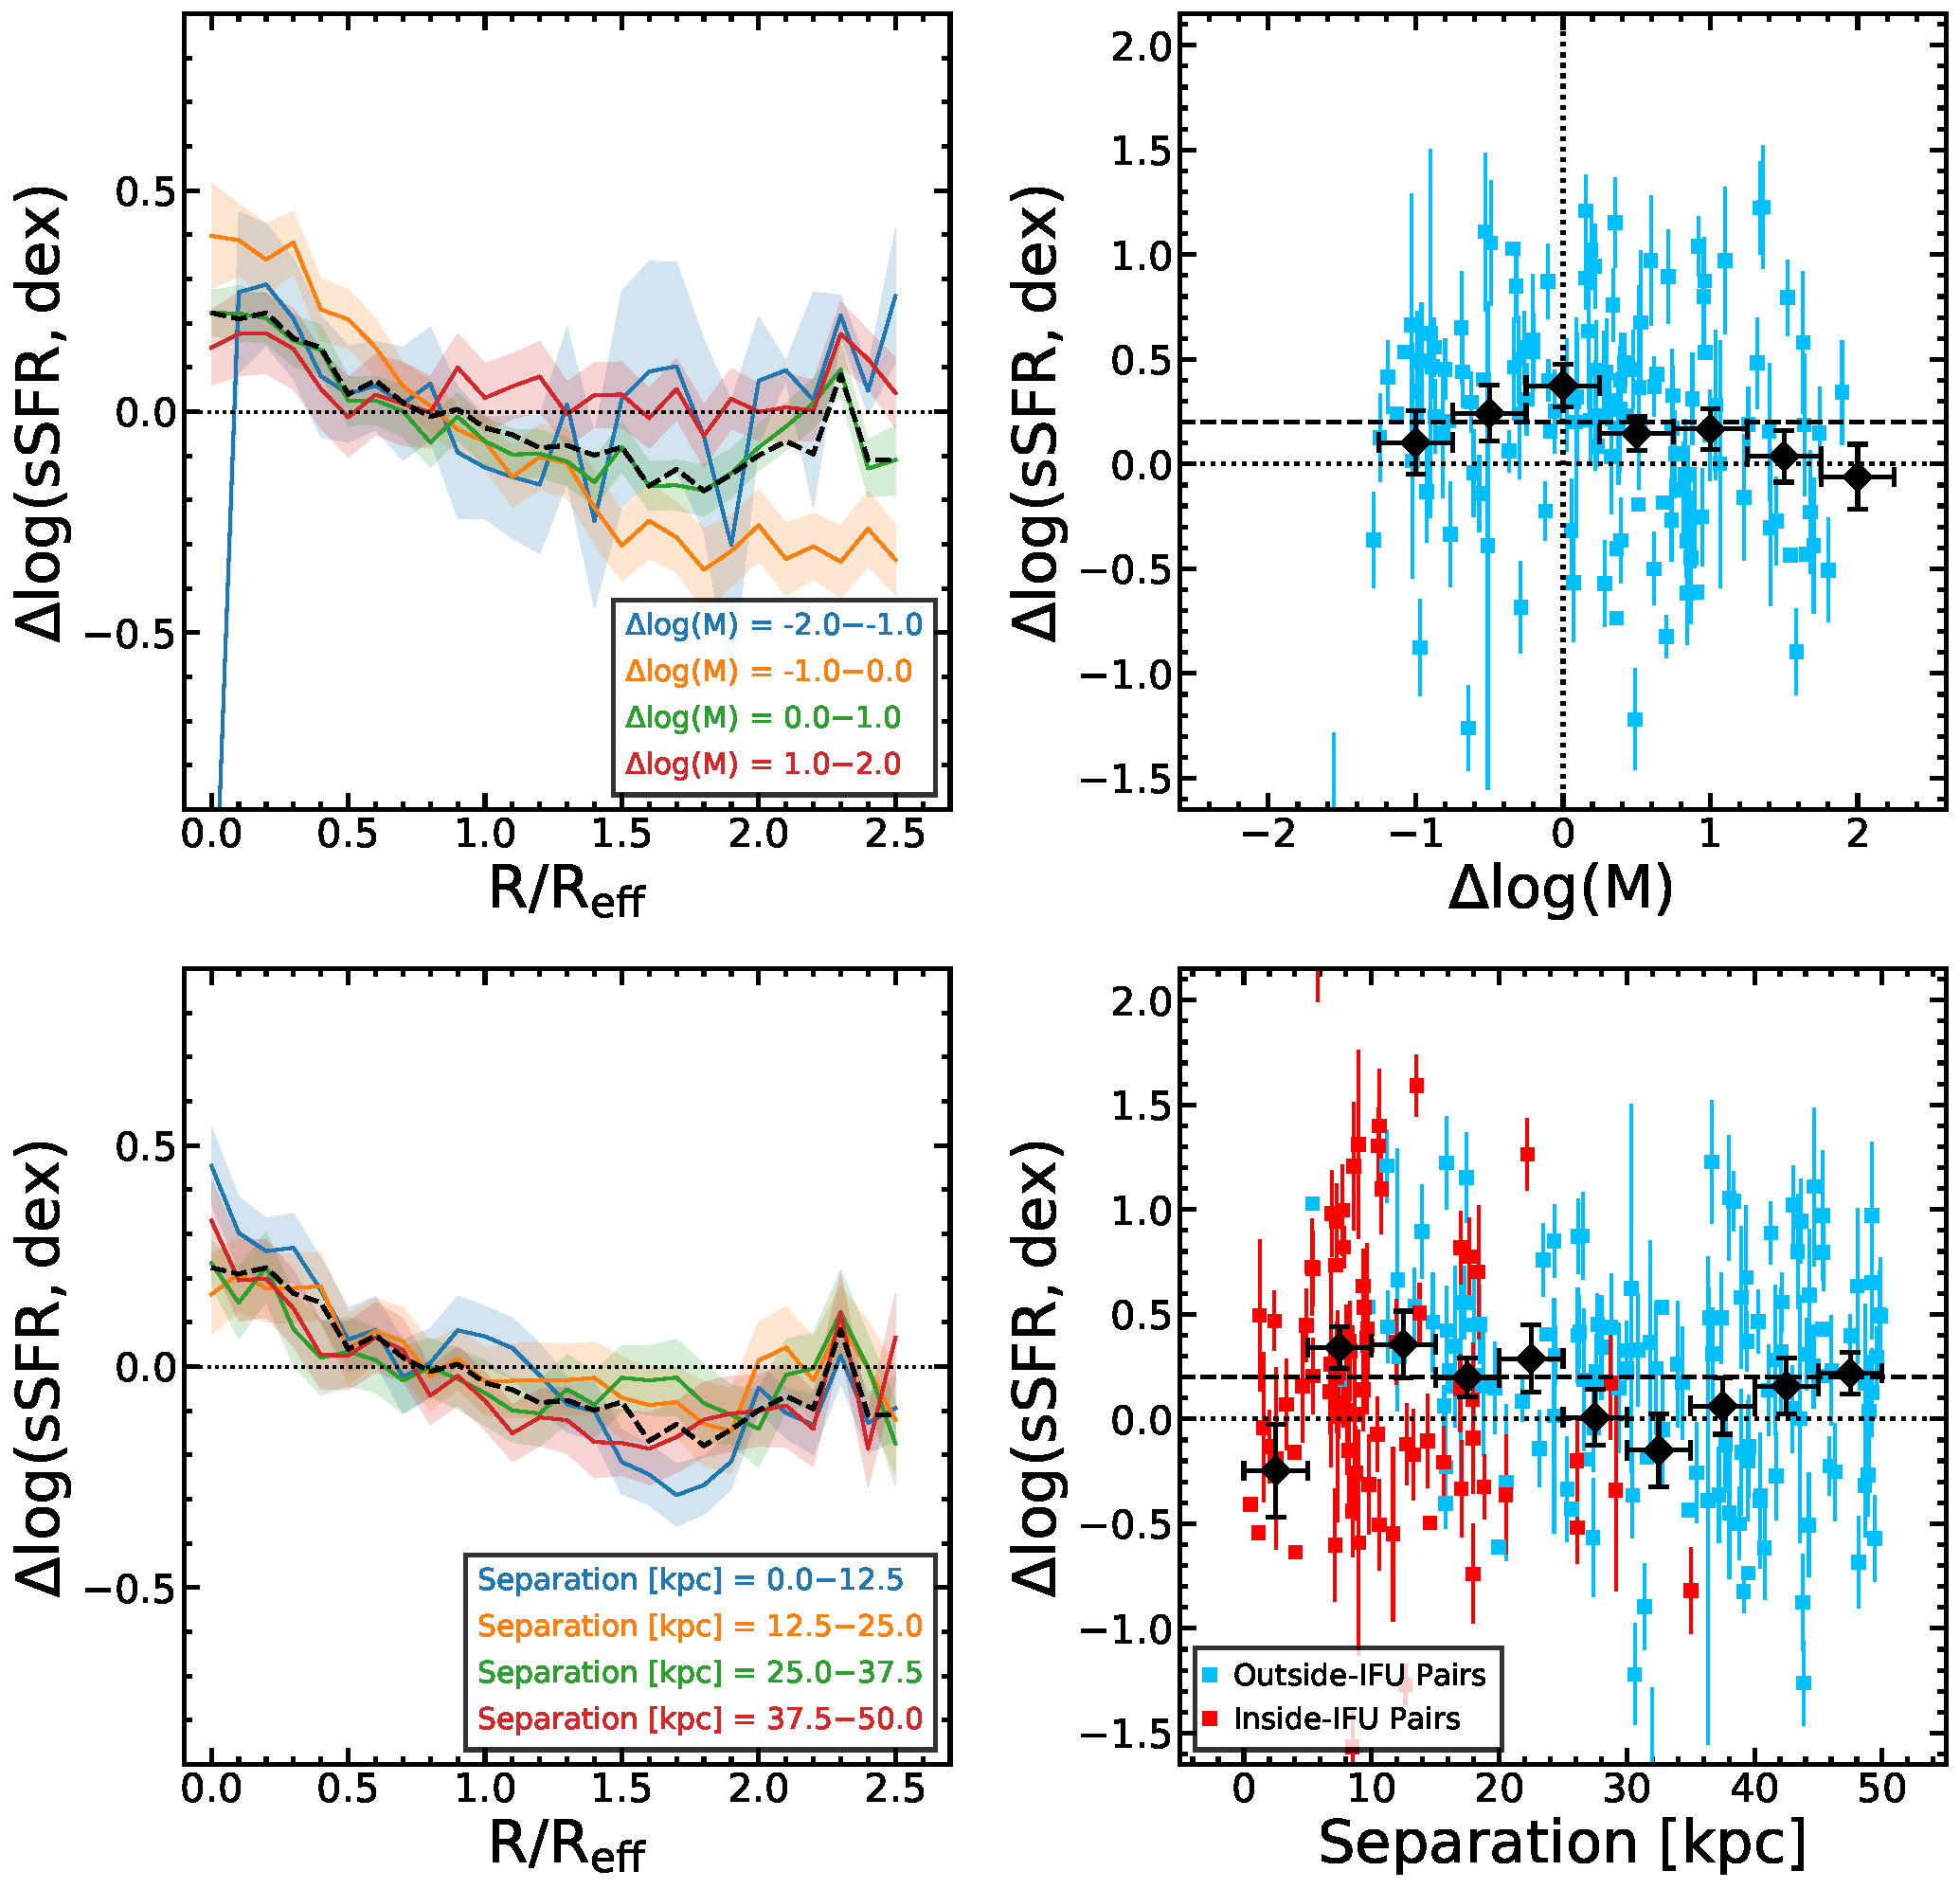
\includegraphics[width=\linewidth]{fig/ssfr_partial.pdf}
\caption[]{{\it Use larger bins here.} Same as Figure \ref{fig:ssfr_mass} except the difference profiles are split by mass ratio (\textbf{Top row}) and projected separation (\textbf{Bottom row}). }
\label{fig:ssfr_dmsep}
\end{figure*}
%%%%%%%%%%%%%%%%%%%%%%%%%%%%%%%%%%%%%%%%%%%%%%

Among the three parameters, stellar mass, mass ratio, and projected separation, the projected separation has the strongest effect on the $\Delta$log(sSFR) enhancement, followed by the mass ratio. From this we see that the paired galaxies with the strongest enhancements to the central sSFR are paired galaxies with 1:1 mass ratios and  which are within 10 kpc. 

Between the splitting the $\Delta$log(sSFR) profile by stellar mass, mass ratio, and projected separation, we see that the general shape of the profile within the inner 1.0 $R$/\reff\ is unchanged. The profile is peaked in the center of the paired galaxies and linearly (in log space) to zero around 1.0 $R$/\reff. Different projected separations and mass ratios may elevate or suppress the level of the enhancement in the profile's center; however, the shape of the profile is largely unchanged.

\subsection{Comparison with Previous Works}

%%%%%%%%%%%%%%%%%%%%%%%%%%%%%%%%%%%%%%%%%%%%%%
\begin{figure}
\centering
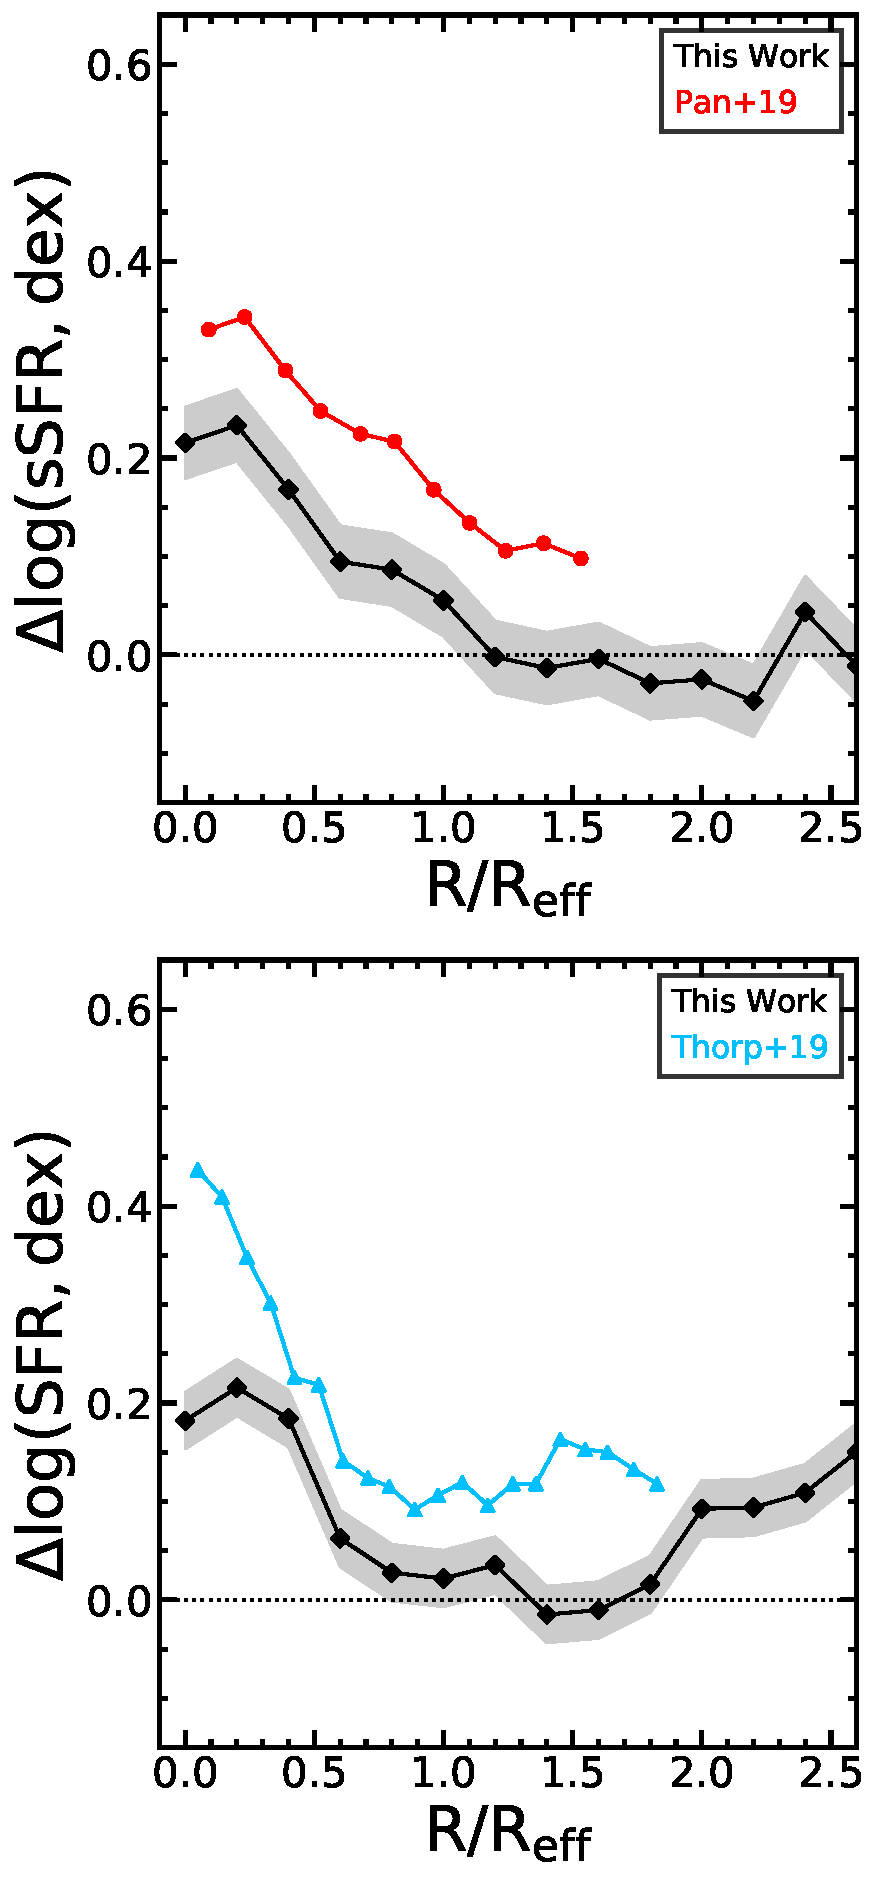
\includegraphics[width=3in]{fig/prof_comp.pdf}
\caption[]{The mean radial profile of $\Delta$log(sSFR) between pairs and controls of this work (Black) compared against those of \citet{Pan:2019} (Red) and \citet{Thorp:2019} (Blue).}
\label{fig:prof_comp}
\end{figure}
%%%%%%%%%%%%%%%%%%%%%%%%%%%%%%%%%%%%%%%%%%%%%%

%%%%%%%%%%%%%%%%%%%%%%%%%%%%%%%%%%%%%%%%%%%%%%
\begin{figure}
\centering
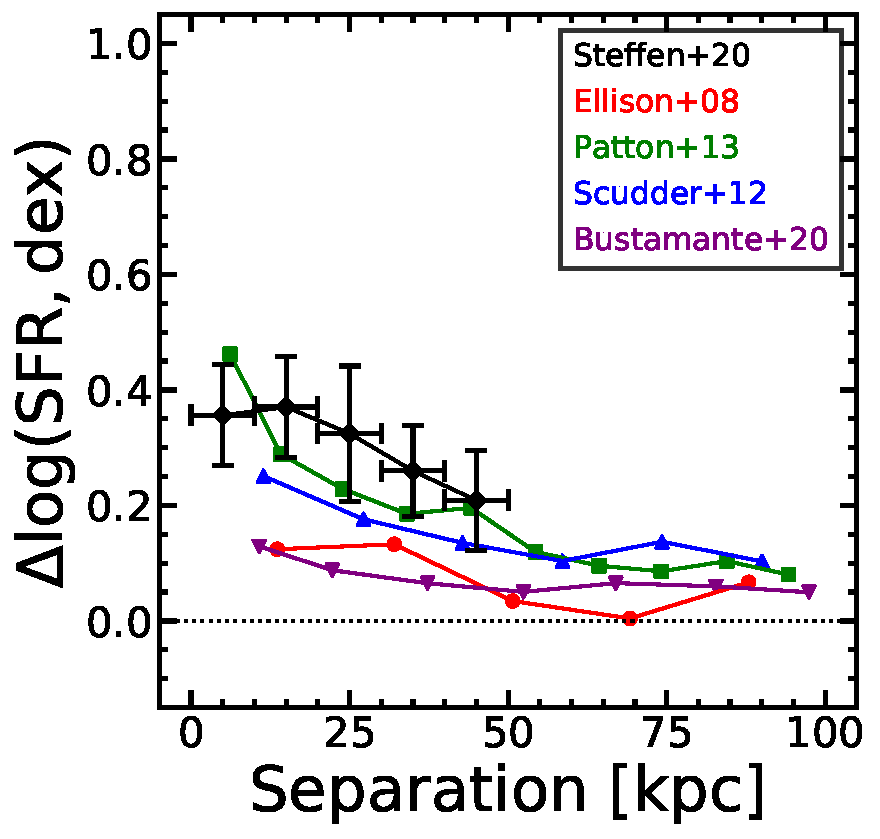
\includegraphics[width=3in]{fig/nuc_sep.pdf}
\caption[]{$\Delta$log(SFR) over projected separation for this sample (Black), \citet{Ellison:2008} (Red), \citet{Li:2008} (Orange), \citet{Scudder:2012} (Blue), \citet{Patton:2013} (Green), and \citet{Bustamante:2020} (Purple).  }
\label{fig:nuc_sep}
\end{figure}
%%%%%%%%%%%%%%%%%%%%%%%%%%%%%%%%%%%%%%%%%%%%%%

\citet{Li:2008} studied the star formation enhancement over different stellar masses and saw that low mass galaxies experience greater levels of enhancement than high mass galaxies.  Galaxies in the mass range \logm\ $=$ 9.72 were shown to experience an enhancement $\sim$0.4 dex higher than galaxies in the mass range \logm\ $=$ 10.6. In this work, we find that $\Delta$log(sSFR) has no dependence on the stellar mass of the galaxy. The galaxies with stellar masses above \logm\ $\ge$ 10.5 do show slightly lower levels of enhancement compared to the lower mass galaxies; however, the pairs still do not significantly deviate from the average $\Delta$log(sSFR) of the sample.

The $\Delta$log(SFR) as a function of projected separation has been studied before with the SDSS survey \citep{Ellison:2008, Li:2008, Patton:2013, Scudder:2012, Bustamante:2020}. We compare the mentioned surveys with our own work in Figure \ref{fig:nuc_sep}. We find that our central SFR enhancements are higher than many of the previous studies, the enhancements are $\sim$0.15 dex higher than \citet{Scudder:2012} and $\sim$0.25 dex higher than \citet{Ellison:2008} and \citet{Bustamante:2020}. The central enhancement to sSFR is $\sim$0.1 dex higher in our pairs compared to \citet{Li:2008} past 35 kpc, but \citet{Li:2008} is $\sim$0.1 dex higher than our pairs at 20 kpc.  Our $\Delta$log(SFR) as a function of projected separation is very consistent to what was found in \citet{Patton:2013}.

Our sample only covers projected separations within 50 kpc, while previous surveys cover out to 100$-$200 kpc. While our sample covers a smaller separation range, the $\Delta$log(SFR) of our sample at 50 kpc is roughly the same level as \citet{Scudder:2012} and \citet{Patton:2013} at the same projected separation. This shows that the central SFR enhancement of our sample is consistent with with what has been found in previous works. 

In Figure \ref{fig:prof_comp} we compare the $\Delta$log(sSFR) profile as a function of galactocentric radius between our work and previous works. \citet{Pan:2019} examines a set of paired galaxies in the MaNGA survey while \citet{Thorp:2019} examines a set of post-merger galaxies in the MaNGA survey. The galaxy pairs in \citet{Pan:2019} have sSFR enhancements that are roughly $\sim$0.1$-$0.2 dex higher than our sample. Our paired galaxies show a slight sSFR suppression in their disks past 1.0 R/\reff\ while the galaxy pairs in \citet{Pan:2019} show an enhancement of $\sim$0.15 dex to the sSFR in their disks. The reason for the discrepancies between our samples is that \citet{Pan:2019} includes a set of post-merger galaxies while our sample has no post-merger galaxies. These post-merger galaxies are predicted to have higher levels of star formation over other paired galaxies due to a second larger burst of star formation which is triggered as the merging galaxies coalesce. 

The post-merger galaxies in \citet{Thorp:2019} have sSFR enhancements between $\sim$0.05$-$0.2 dex higher than our sample of paired galaxies. The centers of the post-merger galaxies feature a greater level of sSFR enhancement in their centers compared to our galaxies pairs of $\Delta$log(sSFR) $=$ 0.5, roughly 0.25 dex higher than our paired galaxies. The post-merger galaxies also feature enhanced sSFR in their disk past 1.0 $R$/\reff\ of $\sim$0.1$-$0.15 dex. The heightened level of sSFR enhancement in the centers of post-merger galaxies in comparison to merging galaxies seems consistent with the idea that a second and greater burst of star formation occurs as the two merging galaxies coalesce into a single galaxy. 

\citet{Barrera-Ballesteros:2015} studied the sSFR in paired galaxies in the CALIFA IFS survey using the H$\alpha$ equivalent width (\ewha) as a proxy for the sSFR. They compared the sSFR in the centers of paired galaxies to their disks by varying the aperture diameters from which they extract the \ewha. They found that the sSFR is enhanced in the centers of the paired galaxies but suppressed in their disks, which is similar to what we find.  


%%%%%%%%%%%%%%%%%%%%%%%%%%%%%%%%%%%%%%%%%%%%%%%%%%%%
\section{Summary and Conclusion}\label{sec:sum}

In this work, we studied a sample of paired, star forming galaxies using the MaNGA IFS survey. We have made a sample of 220 star forming galaxy pairs along with a set of 1891 star forming control galaxies. We compared the radial profiles of the paired galaxies with those of the controls galaxies and found the follwing;

\begin{enumerate}
\item The sSFR is centrally enhanced within the inner 1.0 R/\reff\ by 0.25 $\pm$ 0.1 dex. 
\item The disks of the paired galaxies, R/\reff\ $=$ 1.0$-$2.5, show limited suppression in their disks, $\sim$0.1 dex.
\item The sSFR enhancement in paired galaxies is independent of the total stellar mass of the paired galaxies, Massive galaxies experience the same level of sSFR enhancement as low mass galaxies.
\item The sSFR enhancement in paired galaxies does depend on the ratio between the masses of the paired galaxies. Galaxies with small mass ratios, $|\Delta$log(M)$|$ $=$ 0.0$-$0.5, see an enhancement to sSFR of 0.3 $\pm$ 0.1 dex, which is 0.1 dex higher than the average paired galaxies in the survey. We have also showed that paired galaxies with large mass ratios, $|\Delta$log(M)$|$ $=$ 1.0, still show substantial levels of enhancement to the sSFR, 0.15$-$0.2 dex. 
\item Further, in paired galaxies with large mass ratios, the less massive galaxies experience higher levels of sSFR enhancement than the more massive galaxy in the pair, $\sim$0.1 dex.
\item The sSFR enhancement increases with closer projected separations where galaxies within 5$-$15 kpc have their sSFR enhanced by 0.3$-$0.4 $\pm$ 0.1 dex. 
\item When splitting the sSFR enhancement profiles by stellar mass, mass ratio, or projected separation, the general shape of the enhancement profile is unchanged. While lower projected separations or mass ratios closer to 1:1 may raise the level of the central enhancement to the profiles, the profiles still linearly fall to zero enhancement around 1.0 R/\reff\ with roughly the same gradient.
\item The paired galaxies will experience a fractional mass growth rate of 1$-$6\%, where the growth in mass in largest in low mass galaxies.

\end{enumerate}

\acknowledgments

% funding
J.S. and H.F. acknowledge support from the National Science Foundation (NSF) grant AST-1614326. Funding for the Sloan Digital Sky Survey IV has been provided by the Alfred P. Sloan Foundation, the U.S. Department of Energy Office of Science, and the Participating Institutions. SDSS acknowledges support and resources from the Center for High-Performance Computing at the University of Utah. The SDSS web site is www.sdss.org.

SDSS is managed by the Astrophysical Research Consortium for the Participating Institutions of the SDSS Collaboration including the Brazilian Participation Group, the Carnegie Institution for Science, Carnegie Mellon University, the Chilean Participation Group, the French Participation Group, Harvard-Smithsonian Center for Astrophysics, Instituto de Astrofísica de Canarias, The Johns Hopkins University, Kavli Institute for the Physics and Mathematics of the Universe (IPMU) / University of Tokyo, the Korean Participation Group, Lawrence Berkeley National Laboratory, Leibniz Institut für Astrophysik Potsdam (AIP), Max-Planck-Institut für Astronomie (MPIA Heidelberg), Max-Planck-Institut für Astrophysik (MPA Garching), Max-Planck-Institut für Extraterrestrische Physik (MPE), National Astronomical Observatories of China, New Mexico State University, New York University, University of Notre Dame, Observatório Nacional / MCTI, The Ohio State University, Pennsylvania State University, Shanghai Astronomical Observatory, United Kingdom Participation Group, Universidad Nacional Autónoma de México, University of Arizona, University of Colorado Boulder, University of Oxford, University of Portsmouth, University of Utah, University of Virginia, University of Washington, University of Wisconsin, Vanderbilt University, and Yale University.

%%%%%%%%%%%%%%%%%%%% REFERENCES %%%%%%%%%%%%%%%%%%
\bibliographystyle{aasjournal}
\bibliography{mergerbib}

%%%%%%%%%%%%
% Appendix
%%%%%%%%%%%%

%\hbox{}\clearpage

%\appendix

%\section{Figures}

\end{document}